Para iniciar el sistema se paso de modo real a modo protegido, para ello necesitamos establecer una GDT que nos delimite los distintos segmentos a usar por nuestro kernel.\\

Por enunciado se pedian 5 descriptores, 1 de video, codigo de nivel kernel, datos de nivel kernel, codigo de nivel usuario y datos de nivel usuario. Se definio por cada entrada un indice (en orden del 18 al 22) y un descriptor:

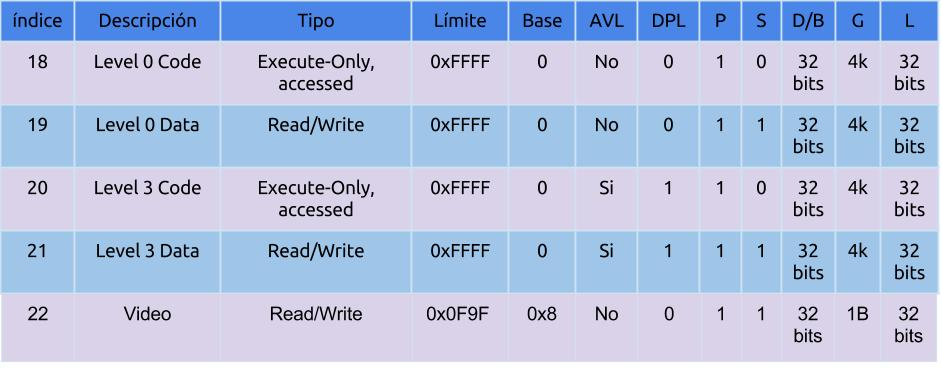
\includegraphics[scale=0.4]{diagramas/gdt-primerasEntradas.jpg} 
\\Organizacion de la GDT: primeras entradas.\\

Una vez completa, se incluyo en el codigo del kernel la instruccion LGDT para cargar en el procesador la direccion de memoria de la misma. Paso seguido seteamos el bit 0 del registro CR0 en 1 para pasar al modo protegido y efectuamos un salto para hacer que el procesador se setee en el segmento de codigo de kernel, indice 18 de la GDT con la instruccion JMP 0x90:protected$\_$mode. Se utiliza el valor 0x90 para saltar al segmento correspondiente ya que el indice del segmento al que necesitamos ir (codigo de kernel) es el 18$_10$. Como el RPL es 0 de kernel y estoy accediendo a una entrada de la GDT, los 3 primeros bits del selector son 0, equivalente de multiplicar por 8: 18$_10$ x 8$_10$ = 0x90

Despues seteamos los registros selectores a los segmentos correspondientes e inicializamos la pila del kernel en la posicion 0x27000, pasandole este valor al registro ESP y EBP.



\lstinputlisting[tabsize=4, numbers=left, numberstyle=\tiny\color{black},mathescape=true, backgroundcolor=\color{gray}, rulecolor=\color{black}, keywordstyle=\color{blue}, commentstyle=\color{dkgreen},stringstyle=\color{mauve}, numbersep=5pt, basicstyle=\scriptsize]{diagramas/kernel.asm}
